%!TEX root = ../master.tex
\chapter{Fundamentals of Learning Theory}\label{chap_fundamentals_learning}


\begin{theorem}
	Learning theory is an important part of aligning students' mental model with the real world. Knowing how engineering students learn becomes a vital part of designing a learning activity and a learning object.
\end{theorem}

\noindent
Learning can include a wide variety of different activities such as reading a chapter of a book, listening to a presentation, having a discussion, taking notes, browsing the Internet, seeing a demonstration, playing a game, etc. There are many different ways of learning, and the learning activity that individuals get the most out of may vary. \\

\noindent
Designing a learning activity involves three elements (Figure~\ref{fig:course_triangle}): learning outcomes, means (hence the teaching methods and learning experience), and the assessment tasks \cite[p. 7]{potter2012primer}. The learning outcome determines the student's desired achievement, the teaching and learning experiences must be designed to achieve the desired outcome, and the assessment task evaluates to what degree the outcome has been achieved.

\begin{figure}[H]
\centering
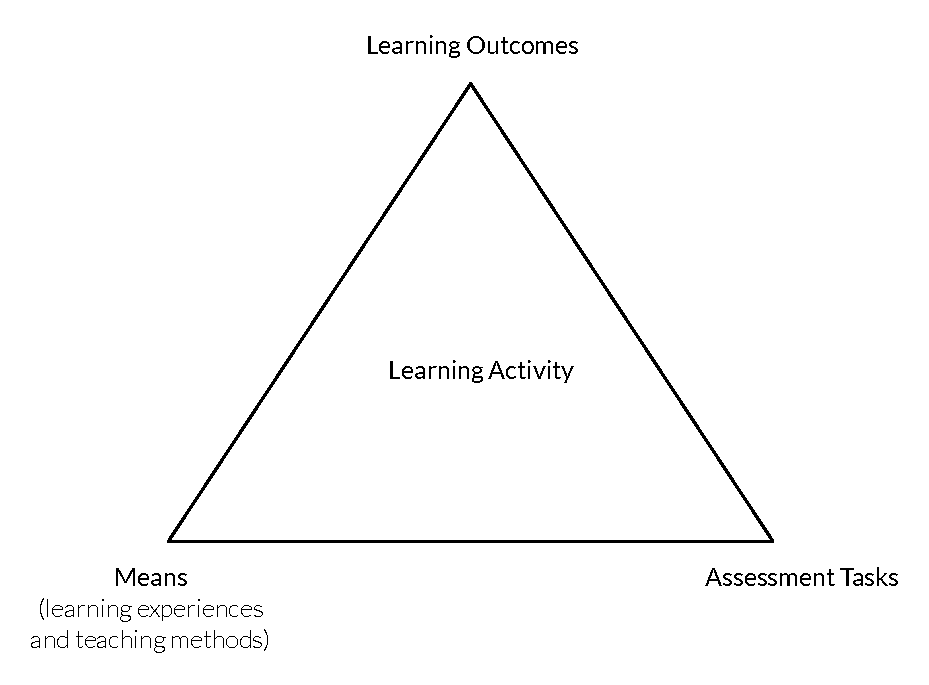
\includegraphics[width=8cm]{figures/course_triangle}
\caption{Essential Components in a Learning Activity \cite[p. 7]{potter2012primer}}
\label{fig:course_triangle}
\end{figure}

\noindent 
The following two sections cover the design of learning outcomes and assessment tasks described with Bloom's and SOLO taxonomies. The subsequent sections cover the means using learning theories.
\begin{citat} []
The teaching methods are the means; the learning outcomes are the ends \textbf{- Potter and Kustra, 2012} \cite[p. 7]{potter2012primer}
\end{citat}

\section{Bloom's Taxonomy}

In 1956 Bloom, Engelhart, Furst, Hill, and Krathwohl, published a new taxonomy, Bloom's taxonomy. The purpose of the taxonomy was to \textit{"promote higher forms of thinking in education"} \cite[p. 1]{clark2015blooms}. The original taxonomy included six major categories in the cognitive domain; \textit{Knowledge}, \textit{Comprehension}, \textit{Application}, \textit{Analysis}, \textit{Synthesis}, and \textit{Evaluation} \cite[p. 212]{krathwohl2002revisedbloom}. The ordering of categories are in the degree of difficulty, that is, one must normally be mastered before the next. Bloom's taxonomy has most frequently been used to classify curricular objectives and assess students to verify whether or not the objectives are met.\\

\noindent
A revision of Bloom's taxonomy was published in 2001 by a former student of Bloom, Anderson, and Krathwohl. The revision included a change of the six categories from nouns to verbs. Further, a rearrange of the Evaluation and Synthesis steps in the original taxonomy was implemented. \textit{"The new taxonomy reflects a more active form of thinking and is perhaps more accurate"} \cite[p. 4]{clark2015blooms} The revision also introduced an extra dimension that in the original taxonomy was hidden in the subcategories. Hence, the revised version contains the Cognitive dimension (box below) and the  Knowledge dimension, which includes; Factual Knowledge, Conceptual Knowledge, Procedural Knowledge, and Metacognitive Knowledge \cite[p. 214]{krathwohl2002revisedbloom}.

\begin{kasse}[Bloom's Revised Taxonomy]
\textit{"Structure of the Cognitive Process Dimension of the Revised Taxonomy"} \cite[p. 215]{krathwohl2002revisedbloom}

\begin{itemize}
\setlength\itemsep{0.05em}
  \item \textbf{Remember} - Retrieving relevant knowledge from long-term memory
  \item \textbf{Understand} - Determining the meaning of instructional messages, including oral, written, and graphic communication
  \item \textbf{Apply} - Carrying out or using a procedure in a given situation 
  \item \textbf{Analyze} - Breaking material into its constituent parts and detecting how the parts relate to one another and to an overall structure or purpose
  \item \textbf{Evaluate} - Making judgments based on criteria and standards
  \item \textbf{Create} - Putting elements together to form a novel, coherent whole or make an original product.
\end{itemize}
\end{kasse}


\noindent 
Bloom's taxonomy gives teachers, instructors, and educators a convenient way to describe the degree to which they want their students to understand and use concepts, to demonstrate particular skills, and to have their values, attitude, and interests affected.

\section{SOLO Taxonomy}

In 1982, Biggs and Collis described a taxonomy they named SOLO. SOLO stands for \textbf{S}tructure of \textbf{O}bserved \textbf{L}earning \textbf{O}utcomes and describes the increasing complexity in a student's understanding of a subject through five stages.
Potter and Kustra describe SOLO as: \textit{"Understanding is conceived as an increase in the number and complexity of connections students make as they progress from incompetence to expertise"} \cite[p. 9]{potter2012primer}.
The difference between SOLO taxonomy and Bloom's taxonomy is according to Biggs and Collis: \textit{"Bloom Taxonomy is really intended to guide the selection of items for a test rather than to evaluate the quality of a student's response to a particular item"}, and mention that this \textit{"makes it difficult to apply the Taxonomy meaningfully to open-end responses"} \cite[p. 13]{biggs1982evaluating}. Whereas SOLO, on the other hand, is designed for assessing open-ended responses. \\

\noindent
SOLO and Bloom's taxonomy are not mutually exclusive, and can be used in conjunction to design curriculums in terms of intended learning outcomes and assessments of learning outcomes. \\

\noindent
The five stages in SOLO taxonomy (Figure~\ref{fig:solo_taxonomy}) are: pre-structural, unistructural, multistructural, relational, and extended abstract.

\begin{figure}[H]
\centering
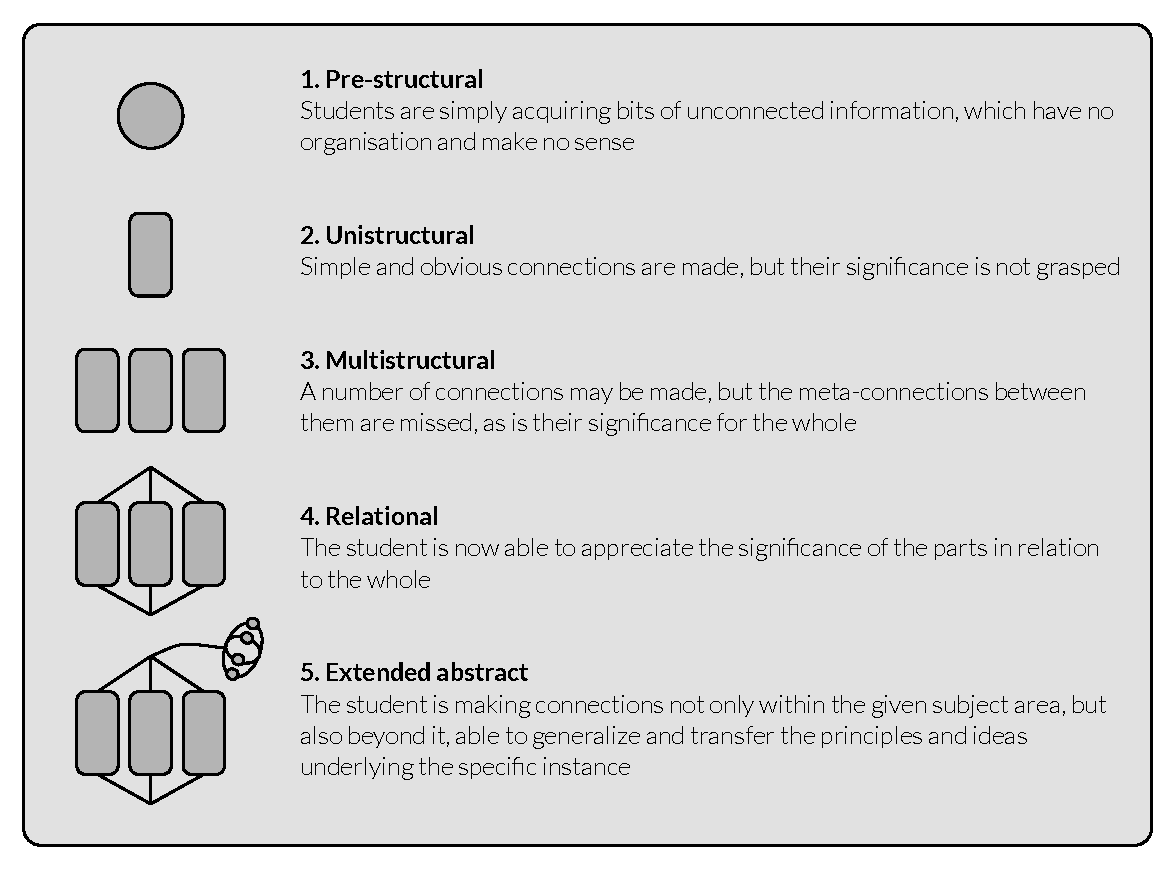
\includegraphics[width=\textwidth]{figures/solo_taxonomy}
\caption{Stages in SOLO Taxonomy \cite{atherton2013solo}}
\label{fig:solo_taxonomy}
\end{figure}

\noindent 
The pre-structural stage in SOLO taxonomy refers to a stage of ignorance, where the presented information barely makes any sense. An example of an answer to the question of \textit{"Why use the SOLO taxonomy to create learning outcomes?"} from a student in the pre-strucrutal stage could be: \textit{"I don't know"} \cite[p. 10]{potter2012primer}. \\

\noindent
 The two following stages, unistructural and multistructural, are typically described to be levels of superficial understanding, in which simple and obvious connections are made. The significance of the connections is not fully grasped.
An example of an answer from a student in the unistrucrutal stage could be: \textit{"It helps you choose appropriate expectations"} \cite[p. 11]{potter2012primer}. The multistructural level refers to a few numbers of additional connections made compared to the unistructural level, but the significance is still not grasped. A deep understanding of a topic can be achieved, but without connections to other topics, "the big picture" is still missing. 
An example of an answer from a student in the multistrucrutal stage could be: \textit{"It helps you choose appropriate expectations, plan an assessment strategy, organize a useful sequence of learning experiences, and use outcomes to encourage deeper approaches to learning"} \cite[p. 12]{potter2012primer}. \\

\noindent
The last two stages in SOLO taxonomy refers to the understanding and grasping of the concepts and abstractions. The first and last stages of SOLO taxonomy can be viewed as existing outside of the learning activity. The pre-structural stage refers to the knowledge prior to entering the learning experience, whereas the extended abstract stage relates to the usage of the knowledge gained after the end of a learning activity. An important fact to remember is that students go through this learning cycle iteratively within each topic the instructor introduces. The student may be at different levels of SOLO taxonomy within the different subjects of the curriculum.

\section{Learning and Teaching Styles}
\label{section:learning_styles}

There are different styles of learning - and students learn in a variety of ways. To mention a few; seeing, hearing, reflecting, experimenting, acting, memorizing, and visualizing. Likewise, there exist many different styles of teaching. Extensive research with a focus on optimizing students' learning outcome both in general and specialized areas of education has been carried out. Felder and Silverman described in 1988 a mismatch between learning and teaching styles in engineering education \cite[p. 674]{Felder88k.:learning}. In the following section, we will discuss how engineering students learn and discuss the teaching methods matching these styles of learning.

\subsection*{Learning Styles}
Felder and Silverman define a learning style model that \textit{"classifies students according to where they fit on a number of scales pertaining to the ways they receive and process information"} \cite[p. 674]{Felder88k.:learning}. They propose a conceptual framework of 32 different learning styles in their original article, based on among others Jung's theory of psychological types. However, the article went through a revision 14 years after its first publication in 1988 with two significant changes in the model. The revised model removes the category of inductive and deductive learning from the original model because of extensive research suggesting that induction is the "best" method of learning. Induction refers to styles such as problem-based learning which will be covered later in this chapter. The original article defined a Visual and Auditory category, which was changed to Visual and Verbal to include both written and spoken words in the verbal category.  

\begin{kasse} [Model of Learning Style \cite{Felder88k.:learning}]
A summary of the four questions in the revised version to answer in order to define a student's learning style:
\vspace{-3mm}
\begin{itemize}
  \setlength\itemsep{0.05em}
  \item \textit{What type of information does the student preferentially perceive?}
  \vspace{-3mm}
  \begin{itemize}
  \setlength\itemsep{0.05em}
  \item \textbf{Sensory} (external): Sights, sounds, physical sensations
  \item \textbf{Intuitive} (internal): Possibilities, insights, hunches
\end{itemize}
\item \textit{Through which sensory channel is external information most effectively perceived?}
\vspace{-3mm}
\begin{itemize}
  \setlength\itemsep{0.05em}
  \item \textbf{Visual}: Pictures, diagrams, graphs, demonstrations
  \item \textbf{Verbal}: Spoken and written words, sounds 
\end{itemize}
\item \textit{How does the student prefer to process information?}
\vspace{-3mm}
\begin{itemize}
  \setlength\itemsep{0.05em}
  \item \textbf{Actively}: Through engagement in physical activity or discussion
  \item \textbf{Reflectively}: Through introspection
\end{itemize}
\item \textit{How does the student progress toward understanding?}
\vspace{-3mm}
\begin{itemize}
  \setlength\itemsep{0.05em}
  \item \textbf{Sequentially}: In continual steps
  \item \textbf{Globally}: In large jumps, holistically
\end{itemize}
\end{itemize}
\end{kasse}

\noindent 
The revised version defines 16 different combinations of learning styles. To focus our efforts towards the majority of preferences in learning style, we need to understand which styles are most dominant.

\subsubsection*{Sensing and Intuitive Learning}
Sensing and Intuitive learning refer to the two ways in which people tend to perceive the world. \textit{"Sensing involves observing, gathering data through senses"}  \cite[p. 676]{Felder88k.:learning} whereas \textit{"intuition involves indirect perception by way of the unconscious -- speculation, imagination, hunches"} \cite[p. 676]{Felder88k.:learning}. \textit{"Sensors like facts, data and experimentation"} \cite[p. 676]{Felder88k.:learning} whereas \textit{"intuitors prefer principles and theories"} \cite[p. 676]{Felder88k.:learning}. Felder and Silverman's research suggests that
the primary focus is on lectures and readings instead of facts and practical exercises. They point out a mismatch in the style of teaching that favors intuitive learners whereas the majority of engineering students have a preference of a sensory learning style. The learning activity should reach both types, to embrace engineering students' learning styles. Targeting the learning activity can be done by blending concrete information such as facts, data, and observable phenomena with abstract concepts such as principles, theories, and mathematical models. 

\subsubsection*{Visual and Verbal learning}
Visual and Verbal refer to the ways people receive information. Visual involves sights, pictures, diagrams, symbols, etc. whereas verbal involves sounds and words (both written and spoken). \textit{"Visual learners remember best what they see"} \cite[p. 676]{Felder88k.:learning}, and verbal learners \textit{"remember much of what they hear and more of what they hear and then say"} \cite[p. 676]{Felder88k.:learning}. Felder and Silverman's research shows that most people of college age and older are visual while most teaching is verbal. To optimize learning to include both types, it is important to include visual material such as pictures, diagrams and sketches accommodating e.g. textual slides.

\subsubsection*{Active and Reflective learning}
Active and Reflective learning refers to \textit{"the complex mental process by which perceived information is converted into knowledge" }\cite[p. 678]{Felder88k.:learning}. Active involves experimentation with the information in the external world whereas \textit{"reflective observation involves examining and manipulating the information introspectively"} \cite[p. 678]{Felder88k.:learning}. Felder and Silverman's research suggests that there are indications that engineers are more likely to be active than reflective learners. By altering lectures with occasional pauses for reflection and brief discussion or problem-solving activities, the learning outcome can be targeted towards both learning style preferences.

\subsubsection*{Sequential and Global learning}
Sequential and Global learning refers to the order that students will learn. Some students are comfortable with the sequential process typically used in universities where \textit{"mastering the material more or less as it is presented"} \cite[p. 679]{Felder88k.:learning}. Others, however, do not learn in this sequential manner, but suddenly they will "get it". Felder and Silverman describe the global learners as: \textit{"They may then understand the material well enough to apply it to problems that leave most to the sequential learners baffled"} \cite[p. 679]{Felder88k.:learning}. Basically, sequential learners follow linear reasoning when solving problems whereas global learners make intuitive leaps. To address both types of students, instructors should provide "the big picture" or goal of the lesson to reach the global learners. \\

\noindent
Felder and Silverman's research shows that engineering students prefer \textbf{sensory}, \textbf{visual}, \textbf{active}, and \textbf{sequential} learning styles \cite[p. 680]{Felder88k.:learning}.


\subsection*{Teaching Styles}
The previous section defined the learning style preferences of engineering students, and what instructors can do to address the individual types. Looking at teaching styles from a higher perspective reveals two main approaches to teaching; teacher-centered approach, and student-centered approach.
 
\subsubsection*{Teacher-Centered Approach}
The teacher-centered approach to learning has the teacher as the main figure of authority. The student is passive and viewed as an \textit{"empty vessel"} \cite{teaching_methods} that has to be filled with knowledge via lectures or direct instruction. The goal of a learning approach with a teacher-centered approach is a test with an assessment based on e.g. a scored test. 

\subsubsection*{Student-Centered Approach}
In contrast to the teacher-centered approach, the focus is shifted to include the students to a greater extent. The role of the instructor shifts to a more coaching and facilitating role. The student-centered approach connects teaching and assessment and students are continuously evaluated by doing group projects, class participation, presentations, etc. \\

\noindent
The relation between engineering education and the learning style/teaching approaches are summed up in Felder's revision notes to the original article. Felder describes that \textit{"the 'best' method of teaching"} (at least below graduate school level) \cite{Felder88k.:learning} is a student-centered approach, like problem-based learning as we will discuss in the following section. Furthermore instructors within engineering education need to focus on teaching styles that match the most prefered learning styles.


\section{Problem-Based Learning}

Problem-Based Learning (PBL) is a student-centered approach to learning. PBL was invented by Dr. Barrows in the 1960s in an attempt to \textit{"solve a problem he encountered while teaching medical students: they did not remember what they had learned and did not use reasoning processes characteristic of physicians"} \cite[p. 1]{walker2015essential}. 

\begin{definition} [Problem-Based Learning]
Problem-Based Learning is an instructional (and curricular) learner-centered approach that empowers learners to conduct research, integrate theory and practice, and apply knowledge and skills to develop a viable solution to a defined problem. \cite[p. 7]{walker2015essential}
\end{definition}

\noindent
PBL facilitates problem-solving and is centered around a specific real-world problem with no single correct answer. PBL enforces group work and self-learning in order to solve the problem and apply new knowledge, and reflect on the learning outcome. Furthermore, the instructor's role is to \textit{"facilitate the learning process rather than to provide knowledge"} \cite[p. 235]{hmelo2004pbl}. The box below sums up the main goals of PBL.

\begin{kasse} [The Goals of Problem-Based Learning]
\textit{"PBL was designed to help students"} \cite[p. 240]{hmelo2004pbl}
\begin{itemize}
  \setlength\itemsep{0.05em}
  \item construct an extensive flexible knowledge base
  \item develop effective problem-solving skills
  \item develop self-directed, lifelong learning skills
  \item become effective collaborators
  \item become intrinsically motivated to learn
\end{itemize}

\end{kasse}

\noindent
Problem-based approaches have been used for many years, and Santos and Monte point out the relevance to software engineering education. 
\textit{"Given the demand [...] for solutions that actually contribute to modern organizations, the search for qualified professionals who have considerable practical experience has been growing day by day"} \cite[p. 1]{santos2013pbl}. Furthermore, Santos and Monte describe, and set out to investigate the effectiveness of, how PBL can improve the skill set of software engineers.
\textit{"PBL have merged in higher education as an approach to foster changes in teaching and learning processes, which are aligned to the new requirements of the labour market"} \cite[p. 1]{santos2013pbl}.


\section{Activity-Based Learning}

Activity-based learning (ABL) is an approach that has elements similar to PBL incorporated. The approach focuses on the activity-first, instead of the problem-first approach as in PBL. Churchill describes the goal of activity-based learning as the construction of \textit{"mental models that allow for 'higher-order' performance such as applied problem solving and transfer of information and skills"} \cite[p. 1]{churchill2003effective}. Fallon, Eimear and Walsh point out the outcome of activity-based education as students become \textit{"more actively involved in the learning process through acts of 'doing', 'being' and 'critically reflecting' than in traditional, didactic education that is more centered around the passive act of 'knowing'"} \cite[p. 4-5]{fallon2013activity}. \\

\noindent The following sections will describe some of the theories behind these ABL approaches and how learning objects can be an important part of designing a learning experience.


\subsection*{Activity Theory}
Activity theory is a \textit{"philosophical framework for studying different forms of human praxis as developmental processes, both individual and social levels interlinked at the same time"} \cite[p. 62]{jonassen1999activitytheory}. It is a way to analyze and reason about human activity. It is used to analyze activity in many domains such as education, human-computer interaction, activities of everyday living etc. \cite[p. 62]{jonassen1999activitytheory}. In activity theory, activities do not make sense without a context. Engström describes these activities as happening in an \textit{activity system}. 

\begin{figure}
    \centering
    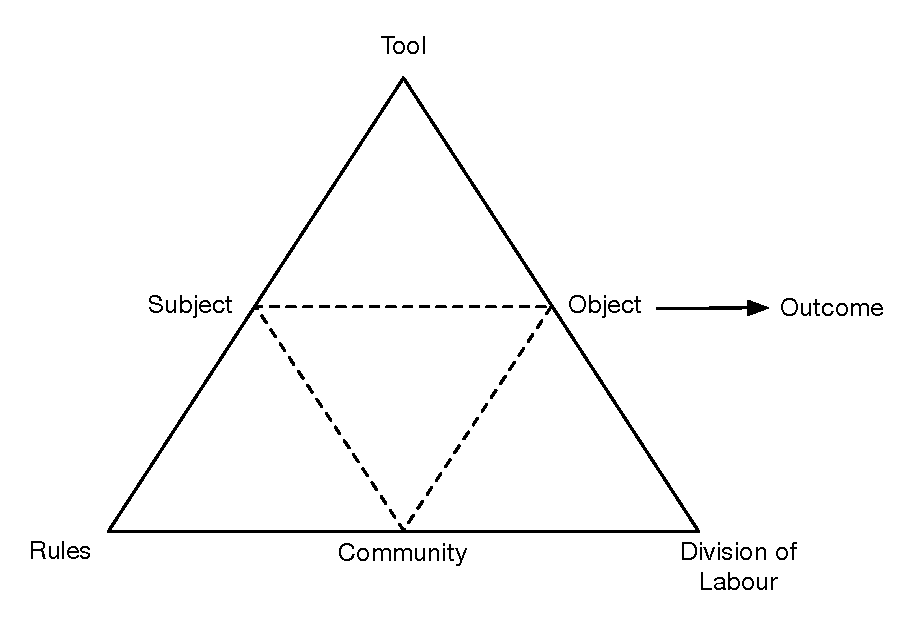
\includegraphics[scale=0.6]{figures/activity_theory}
    \caption{Activity System}
    \label{fig:activity_theory}
\end{figure}


\noindent
Figure \ref{fig:activity_theory} shows Engström's triangle depicting an activity system. The \textit{subject} can be a person or a group, and the \textit{object} is the product of the activity. The object can be physical or mental, and during the activity the object is transformed. \textit{Tools} are what help the subject transform the object and, in the end, reach a given goal. These tools can be physical or mental, for instance a hammer or a model of something. Jonassen describes tools as follows \textit{"Tools can be anything used in the transformation process [...] The use of culture-specific tools shapes the way people act and think"} \cite[p. 63]{jonassen1999activitytheory}. \\

\noindent
The bottom layer contains the constraints of the activity. \textit{Rules} determine what actions and activities the \textit{community} allows e.g. which tools, models, and methods that are used to mediate the process \cite[p. 64]{jonassen1999activitytheory}. \textit{Devision of labor} refers to the division between the individuals in a group who attend to the task in their domain. Designers and developers will, for instance, attend to different areas of the activity. Finally the \textit{outcome} is the end result that can be physical or mental. \\

\noindent
\textit{Tool mediation} is a concept in activity theory about how tools and humans' mental models are connected. Jonassen describes tool mediation as follows: \textit{"tools mediate or alter the nature of human activity and, when internalized, influence humans' mental development"} \cite[p. 66-67]{jonassen1999activitytheory}. Furthermore, the tool cannot be understood without looking at the context of human activity. Nardi \cite[p. 66]{jonassen1999activitytheory} points out that cognitive psychology traditionally ignores artifacts (mediating tools) and says that \textit{"activity cannot be understood without understanding the role of artifacts in everyday existence, especially the way that artifacts are integrated into social practice"}. According to Prawat on tools \textit{"[...] they are looked upon as extensions of the individual"} \cite[p. 39]{postholm2008activitytheory}.


\subsection*{Constructivist Learning Theory}
Constructivist theory is based on Piaget, Dewey, and Vigotsky's view of epistemology: \textit{"There is no knowledge out there independent of the knower, but only knowledge we construct as we learn"} \cite[p. 1]{hein1991constructivist}. From their perspective, learning is not remembered ideas but \textit{"a personal and social construction of meaning out of the bewildering array of sensations"} \cite[p. 1-2]{hein1991constructivist}. \\

\noindent
Piaget did not agree with the earlier educational philosophies on how much value play and exploration would impact learning.
\textit{"Constructivism is relevant in engineering classrooms because of the set of skills learners get to practice and how it helps engineering students build their own knowledge and solutions to problems"} \cite[p. 144]{nino2015constructivist}. McKenna adds to this view in engineering education: \textit{"programming skills are important to help students develop engineering "habits of mind" such as how to break a large complex problem into manageable parts, how to isolate effects, test, and debug problems"} \cite[p. 1]{mckenna2005constructivist}. \\

\noindent
The constructivist learning theory is one of the key epistemological views in problem-based learning.


\subsection*{Learning Objects}

The idea of learning objects has experienced an increase in attraction in the education communities along with the growth of contemporary pedagogies that promote student-based approaches. Churchill proposes a classification of learning objects with the goal of defining the term learning objects in his article \textit{Towards a Useful Classification of Learning Objects} \cite[p. 2]{Churchill2006}.

\begin{kasse} [Types of Learning Objects]
\textit{"Churchill proposes a classification that contains six different types of learning objects:"} \cite[p. 2]{Churchill2006}
\begin{itemize}
    \setlength\itemsep{0.05em}	
  \item \textbf{Presentation object}
      \vspace{-4mm}
      \begin{itemize}
          \item Direct instruction and presentation resources designed with the intention to transmit specific subject matter
    \end{itemize}
    \vspace{-3mm}
  \item \textbf{Practice object}
    \vspace{-4mm}
    \begin{itemize}
          \item Drill and practice with feedback, educational game or representation that allows practice and learning of certain procedures
      \end{itemize}
      \vspace{-3mm}
  \item \textbf{Simulation object}
      \vspace{-4mm}
      \begin{itemize}
          \item Representation of some real-life system or process
    \end{itemize}
    \vspace{-3mm}
  \item \textbf{Conceptual model}    
      \vspace{-4mm}
      \begin{itemize}
          \item Representation of a key concept or related concepts of subject matter
    \end{itemize}
    \vspace{-3mm}
  \item \textbf{Information object}
      \vspace{-4mm}
      \begin{itemize}
          \item Display of information organized and represented with modalities
    \end{itemize}
    \vspace{-3mm}
  \item \textbf{Contextual representation}
      \vspace{-4mm}
      \begin{itemize}
          \item Data displayed as it emerges from represented authentic scenario
    \end{itemize}
\end{itemize}
\end{kasse}

\noindent 
The classifications proposed by Churchill emerge from an extensive amount of attempts to define the term \textit{Learning Object}. He discovers that all types of learning objects appear to have the following common characteristics \cite[p. 4]{Churchill2006}:
\begin{itemize}
  \item they are digital, utilizing different media (and often interactive) to represent data, information, ideas, knowledge, or reality
  \item they are designed to afford educational reuse
\end{itemize}

\noindent Based on the observations above Churchill proposes a general definition of the term \textit{Learning Object}.

\begin{definition} [Learning Object]
\textit{"a learning object is a mediated representation designed to afford uses in different educational contexts"} \cite[p. 4]{Churchill2006}
\end{definition}

\noindent
Learning objects in activity-based theory within engineering education is described by Churchill as: \textit{"Engineering content can effectively be presented with learning objects"} \cite[p. 5]{churchill2003effective}. 
He further argues that \textit{"an active interaction with a learning object [...] enables construction of learners' mental model"} \cite[p.1]{churchill2003effective}. As an example he mentions the use of models of simulating and visualizing objects as digital and interactive models, where the user can change parameters and see the effects of these changes. Churchill describes the use of a learning object as:
\begin{citat} []
If a picture is worth thousands of words, a learning object is worth thousands of pictures. \textbf{- Daniel Churchill, 2003} \cite[p. 5]{churchill2003effective}
\end{citat}


